\documentclass[11pt]{article}

% ---------------------------------------------------------------- packages
\usepackage[margin=1in]{geometry}
\usepackage{graphicx}
\usepackage{booktabs}
\usepackage{amsmath}
\usepackage{caption}
\usepackage{subcaption}
\usepackage{float}
\usepackage[table]{xcolor}
\usepackage{tabularx}
\usepackage{hyperref}
\hypersetup{colorlinks=true, linkcolor=blue!60!black, urlcolor=blue!60!black,
            citecolor=blue!60!black}

% figures live under pipeline/out/figs/ relative to this file
\graphicspath{{pipeline/out/figs/}{figs/}}
\captionsetup{font=small, labelfont=bf}
\newcommand{\R}{$R^2$}

\title{\textbf{Predicting Compressive Strength and Optimal Replacement Level\\
for Rice-Husk-Ash Blended Concrete from a Sparse Literature Dataset}}
\date{\today}

\begin{document}
\maketitle

\begin{abstract}
\noindent
We build a machine-learning pipeline to predict the compressive strength and the
optimal cement-replacement level of rice-husk-ash (RHA) blended concrete, using a
dataset compiled from \textbf{79 research papers}. The central obstacle is data
sparsity: strength values are packed inside free-text cells as
\emph{(replacement level $\times$ curing age)} grids. Parsing and exploding these
cells---rather than any modeling choice---is the highest-leverage step, turning
$\sim$70 packed rows into \textbf{756 clean data
points across 44 papers}. Through a five-axis ablation study we find that
(i)~absolute strength is essentially unpredictable across papers ($R^2<0$) because
the corpus mixes mortars, normal concrete and ultra-high-performance concrete, but
becomes learnable once the paper's own control (0\%) strength is supplied as an
input; (ii)~a strongly-regularized, monotonically-constrained gradient-boosted
model on just three inputs \emph{(replacement, age, control strength)} is the best
predictor, reaching \textbf{\R{}~$=0.50\pm0.20$, MAE~$\approx$~10\,MPa}; and
(iii)~text embeddings (MiniLM/BERT-style) provide \emph{no reliable gain} at this
sample size. The optimal-replacement target cannot yet beat a naive prior---the
derived predictor in fact degenerates to a constant. We conclude that the binding
constraint is data quantity and the absence of base-mix descriptors, not model
capacity.
\end{abstract}

% ============================================================================
\section{Introduction}
Rice husk ash is a pozzolanic by-product that can partially replace Portland cement,
reducing both cost and $\mathrm{CO_2}$ footprint. The two engineering quantities of
interest are the \textbf{compressive strength} of the resulting concrete and the
\textbf{optimal replacement level}---the percentage of cement that can be replaced by
RHA while maximizing strength. Our goal is a predictive model for both, trained on a
dataset hand/LLM-extracted from the literature. The practical difficulties are
(a)~pervasive missing values and (b)~selecting a model that performs well on a small,
heterogeneous dataset. We take XGBoost as the baseline and interrogate the data and
model choices rigorously.

% ============================================================================
\section{The Dataset: What It Actually Contains}
The source file \texttt{RHA Master sheet v2.csv} contains 225 columns organized under
a \textbf{four-row hierarchical header}: category ($\rightarrow$ \textsc{paper
metadata}/\textsc{input}/\textsc{output}), section, feature (55 features), and a
sub-field. Every feature is split into four columns---\texttt{Extracted Value},
\texttt{Unit}, \texttt{Source Type}, \texttt{Exact Evidence}---of which only the first
two carry predictive information; the latter two are provenance and are discarded. The
file is \texttt{latin-1} encoded.

The dataset contains \textbf{79 papers} with unique titles. Sparsity is uneven rather
than uniform: among the 44 papers that yield strength data, availability of the 23
retained features ranges from 96\% (processing method) and 89\% (SiO$_2$) down to 18\%
(BET surface), i.e.\ \textbf{5--82\% missing}, with 8 of the 23 features more than half
missing (Figure~\ref{fig:avail}). The prediction targets are present in 70~(strength),
71~(optimum), and 76~(replacement levels) papers.

\begin{figure}[H]
  \centering
  \begin{subfigure}{0.48\textwidth}
    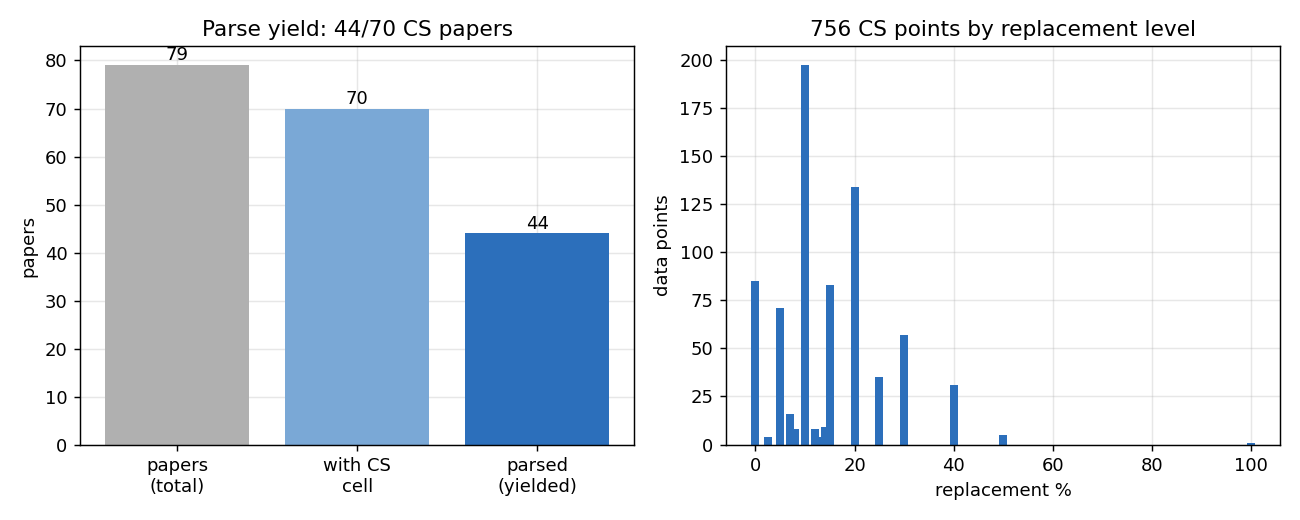
\includegraphics[width=\linewidth]{parse_yield.png}
    \caption{Parse yield and the distribution of recovered strength points by
    replacement level.}
    \label{fig:yield}
  \end{subfigure}\hfill
  \begin{subfigure}{0.48\textwidth}
    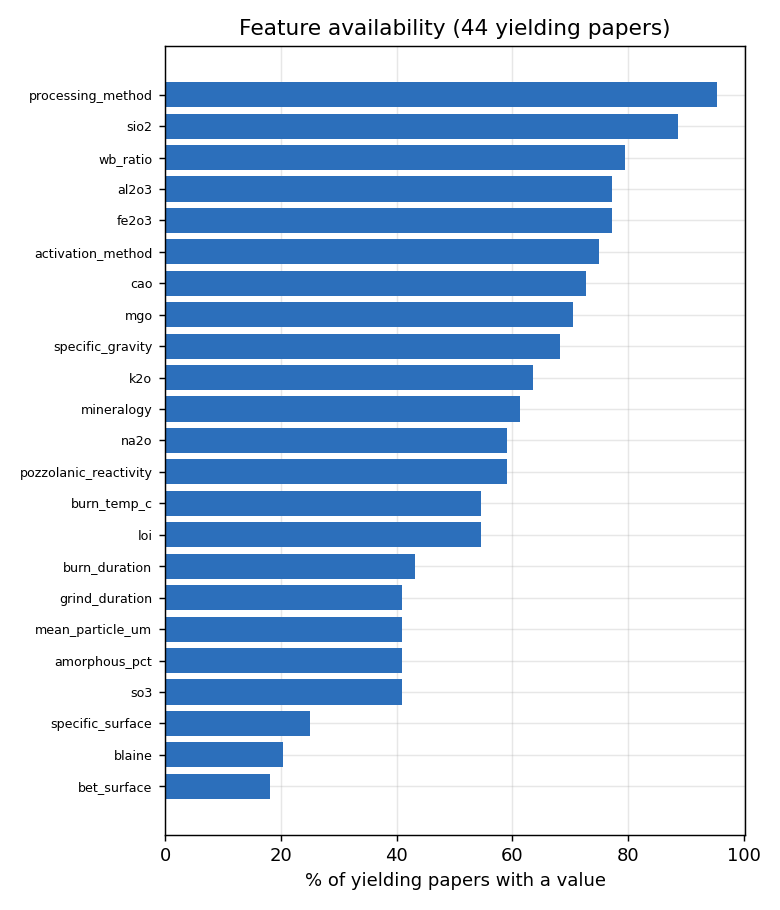
\includegraphics[width=\linewidth]{data_availability.png}
    \caption{Per-feature availability among the 44 yielding papers.}
    \label{fig:avail}
  \end{subfigure}
  \caption{The dataset is small and sparse. Chemistry (SiO$_2$, oxides) and w/b are
  reasonably populated; fineness measures (BET, Blaine, specific surface) are scarce.}
\end{figure}

% ============================================================================
\section{Data Representation: Parsing the Packed Cells}
The single most valuable observation is that each Compressive Strength cell encodes a
\emph{grid} of measurements in one of $\sim$12 textual layouts, e.g.
\begin{quote}\small\ttfamily
3 days: 20 (7\%), 20 (10\%); 28 days: 44.5 (7\%), 46 (10\%); \dots
\end{quote}
We built a state-machine parser (\texttt{02\_parse\_explode.py}) that resolves, for
each value, a \emph{curing age} and a \emph{replacement level} from inline qualifiers,
segment headers, or persistent line context, and emits a tidy long table with one row
per \emph{(paper, replacement\,\%, age)}. Precision safeguards include:
\begin{itemize}\itemsep2pt
  \item unsigned number matching, fixing mis-reads such as \texttt{RHA8-10\%}
        $\rightarrow$ 10 (not $-10$);
  \item a \textbf{per-paper whitelist}: a resolved replacement \% must match the
        paper's declared levels (plus 0 for control), which rejects mis-labelled
        sample IDs (\texttt{RHA1}, \texttt{M2}) and recovers trailing-code mixes
        (\texttt{Aa-10}, \texttt{A35-10});
  \item physical sanity clamps ($0\le\%\le100$, $0<\text{age}\le400$\,d,
        $0.5\le\text{MPa}\le250$).
\end{itemize}
This recovers \textbf{756 data points across 44 of the 70 strength papers} (226 at the
standard 28-day age). The 26 non-yielding papers are graph-derived narratives, pure
ranges, or bare number lists with no age/level mapping---genuinely unrecoverable
without the source PDFs, and logged to \texttt{parse\_failures.csv}.

Figure~\ref{fig:curves} checks the parsed data against expected physics, but both
checks must be made \emph{within} a paper: a raw cross-paper average is dominated by
mix type (the corpus spans 1--205\,MPa), not by the variable of interest. Normalising
each \emph{(paper, replacement level)} series by its own 28-day value, strength does
rise with curing age---91\% of pre-28-day points fall below the series' own 28-day
value and 82\% of later points exceed it, with the median ratio climbing from 0.53 at
1\,d to 1.00 at 28\,d and 1.21 at 90\,d. The strength-vs-replacement shape, by
contrast, is \emph{not} reliably unimodal: of the 33 papers reporting at least three
distinct replacement levels at 28\,d, only 14 (42\%) peak at an interior level, while
12 (36\%) are highest at the lowest level tested---often the 0\% control, meaning RHA
never helped in that paper---and 7 (21\%) are still rising at the highest level tested.
An interior optimum is therefore common but far from universal, which is exactly why
the optimum-prediction task in Section~\ref{sec:opt} is hard.

\begin{figure}[H]
  \centering
  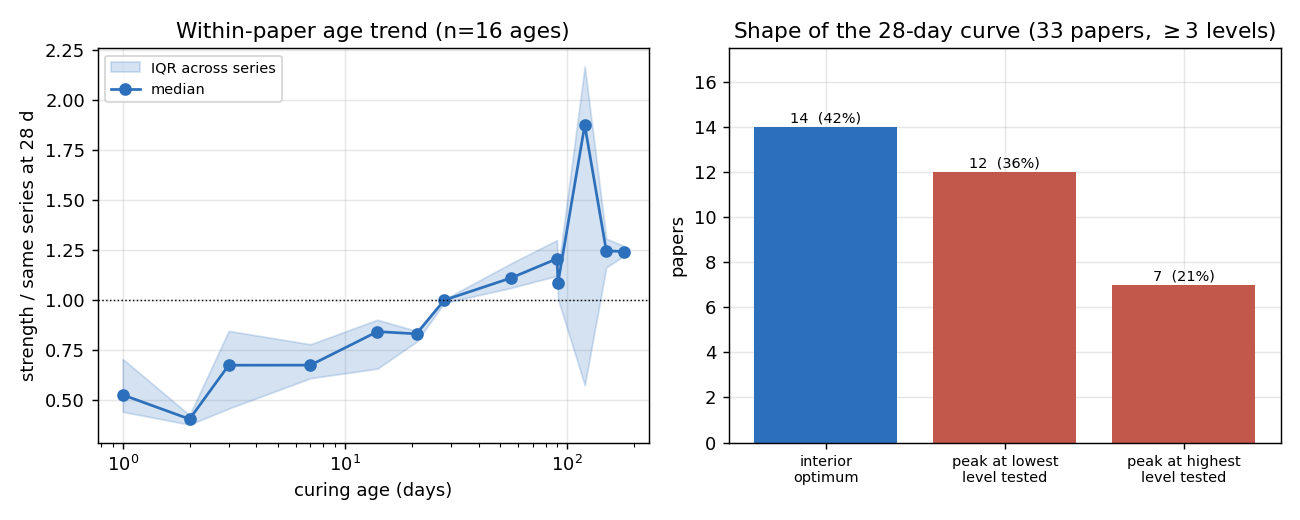
\includegraphics[width=0.9\textwidth]{cs_curves.png}
  \caption{Physics checks on the parsed data, computed within papers. \textbf{Left:}
  each \emph{(paper, replacement level)} series is normalised by its own 28-day
  strength; the median rises with age (shaded band is the IQR across series). Wiggles
  at 2, 91 and 120\,d come from ages with very few series and are small-$n$ noise, not
  a reversal of the trend. \textbf{Right:} the 28-day strength-vs-replacement curve has
  an interior optimum in only 42\% of papers; in 36\% the best level tested is the
  lowest one.}
  \label{fig:curves}
\end{figure}

% ============================================================================
\section{Feature Engineering}
Numeric features (oxides, fineness, w/b, burn temperature/duration) are parsed as the
mean of the numbers in each cell, robustly handling multi-sample entries such as
``94.6 (RHA-A), 93.7 (RHA-B)''. High-cardinality but semantically redundant text
fields are \textbf{canonicalized} into compact categoricals: activation method
$\in\{$none, thermal, mechanical, both$\}$; mineralogy $\in\{$amorphous, mixed,
crystalline$\}$; processing $\in\{$controlled, uncontrolled, \dots$\}$; pozzolanic
reactivity as an ordinal. We deliberately apply \textbf{no imputation} for the
tree models, which handle missing values natively by learning a default split
direction; imputers (median/KNN/MICE) are evaluated separately and only ever fit
\emph{inside} each cross-validation split to prevent leakage.

% ============================================================================
\section{Methodology}
Because rows from the same paper are strongly correlated, all evaluation uses
\textbf{grouped cross-validation by paper}: no paper appears in both training and test.
Given the small sample, a single split is unreliable, so we report the mean and
standard deviation of \textbf{repeated grouped hold-out} (\texttt{GroupShuffleSplit},
30\% of papers held out, 40 repeats). We compare three target framings:
\begin{description}\itemsep2pt
  \item[A. Absolute strength, all papers] predict MPa directly from RHA features.
  \item[B. Relative-to-control] predict strength normalized by the paper's 0\% control.
  \item[C. Absolute strength given control] predict the RHA-blend strength using the
        paper's control (0\%) strength as an additional input---always known in
        practice, hence not leakage. Control rows themselves are excluded from
        evaluation to avoid a trivial identity.
\end{description}

% ============================================================================
\section{Ablation Study}
We ablate five axes. All numbers are repeated grouped hold-out (mean\,$\pm$\,std) over
40 repeats, except the HistGB row of Study~2 and the three imputer rows of Study~4,
where 31 repeats survived (a split is discarded when a held-out fold ends up with no
usable rows). Comparisons \emph{within} a study are like-for-like unless noted.

\paragraph{Study 1 --- Target framing.}
Absolute strength across papers is \emph{unpredictable} (\R{}~$=-0.78$); the corpus
mixes mortars, normal concrete and UHPC (1--205\,MPa) whose baseline levels are set by
mix factors absent from the data. Supplying the control strength (framing~C) makes the
RHA effect learnable (Table~\ref{tab:s1}).

\begin{table}[H]\centering\small
\caption{Study 1: target framing (XGBoost, all structured features).}
\label{tab:s1}
\begin{tabular}{lrrrr}
\toprule
Framing & \R{} & std & RMSE & MAE \\
\midrule
\rowcolor{green!12}C: blend $\mid$ control strength & $0.395$ & $0.259$ & $16.45$ & $10.64$ \\
B: relative-to-control & $-0.159$ & $0.300$ & $0.29$ & $0.22$ \\
A: absolute, all papers & $-0.776$ & $1.549$ & $30.99$ & $20.95$ \\
\bottomrule
\end{tabular}
\end{table}

\paragraph{Study 2 --- Model.}
Random Forest and XGBoost dominate; HistGradientBoosting is unstable and linear
Ridge fails badly on this tiny, collinear, missing-laden matrix
(Table~\ref{tab:s2}). Random Forest posts the higher mean here (0.436 vs 0.395), but
the gap is roughly one-sixth of the run-to-run spread of either model
($\sigma\approx0.21$--$0.26$) and so is not a reliable ordering. We nonetheless carry
\textbf{XGBoost} forward, because the largest single gain in the whole study comes from
the monotone constraints of Study~5 ($0.442\rightarrow0.482$), which XGBoost supports
natively and \texttt{RandomForestRegressor} does not. The tuned monotone XGBoost of
Section~\ref{sec:final} reaches $0.50\pm0.20$, above the unconstrained Random Forest.

\paragraph{Study 3 --- Feature set.}
Parsimony wins decisively: the three-feature \emph{base}
\{replacement, age, control\} is the best set, and \emph{every} added feature group
degrades generalization---clear evidence of overfitting at $n\!=\!23$ papers
(Table~\ref{tab:s3}, Figure~\ref{fig:ablfeat}).

\begin{table}[H]\centering\small
\begin{minipage}{0.46\textwidth}\centering
\caption{Study 2: model (framing C, all features).}
\label{tab:s2}
\begin{tabular}{lrr}
\toprule
Model & \R{} & RMSE \\
\midrule
\rowcolor{green!12}Random Forest & $0.436$ & $15.82$ \\
XGBoost & $0.395$ & $16.45$ \\
Mean baseline & $-0.310$ & $23.97$ \\
HistGB & $-0.524$ & $22.28$ \\
Ridge & $-14.7$ & $44.74$ \\
\bottomrule
\end{tabular}
\end{minipage}\hfill
\begin{minipage}{0.5\textwidth}\centering
\caption{Study 3: feature set (framing C, XGBoost).}
\label{tab:s3}
\begin{tabular}{lrr}
\toprule
Feature set & \R{} & RMSE \\
\midrule
\rowcolor{green!12}base [repl, age, control] & $0.442$ & $15.54$ \\
base + fineness & $0.435$ & $15.73$ \\
base + categorical & $0.427$ & $15.93$ \\
all + MiniLM text & $0.426$ & $16.13$ \\
all + TF-IDF text & $0.403$ & $16.42$ \\
all structured & $0.395$ & $16.45$ \\
base + all numeric & $0.349$ & $16.85$ \\
base + chemistry & $0.317$ & $17.18$ \\
base + processing & $0.236$ & $17.69$ \\
\bottomrule
\end{tabular}
\end{minipage}
\end{table}

\paragraph{Study 4 --- Imputation.}
For the tree models, native NaN handling matches explicit imputation on \R{}: native,
median and KNN sit within 0.007 of one another, and only MICE clearly hurts
(Table~\ref{tab:s4}). The lower RMSE of the median and KNN rows is \emph{not} evidence
that they generalize better---those rows completed 31 of the 40 repeats, so their error
is averaged over an easier subset of splits and is not directly comparable to the
native row's 40. Since no imputer improves \R{} and each adds a fitted component that
must be re-fit inside every split, we keep \textbf{native handling}.

\paragraph{Study 5 --- Physics priors.}
Adding \textbf{monotone constraints}---strength non-decreasing in curing age and in
control strength---gives the single best result, \R{}~$=0.482\pm0.217$, encoding
domain knowledge the tiny sample cannot reliably learn on its own (Table~\ref{tab:s5}).

\begin{table}[H]\centering\small
\begin{minipage}{0.46\textwidth}\centering
\caption{Study 4: imputation (framing C).}
\label{tab:s4}
\begin{tabular}{lrr}
\toprule
Scheme & \R{} & RMSE \\
\midrule
\rowcolor{green!12}XGB + native & $0.397$ & $16.40$ \\
XGB + median$^{\dagger}$ & $0.396$ & $14.88$ \\
XGB + KNN$^{\dagger}$ & $0.390$ & $14.92$ \\
XGB + MICE$^{\dagger}$ & $0.249$ & $16.35$ \\
\bottomrule
\end{tabular}

{\scriptsize $^{\dagger}$31 of 40 repeats; RMSE not comparable to the native row.}
\end{minipage}\hfill
\begin{minipage}{0.5\textwidth}\centering
\caption{Study 5: physics priors (base features).}
\label{tab:s5}
\begin{tabular}{lrr}
\toprule
Prior & \R{} & RMSE \\
\midrule
\rowcolor{green!12}monotone(age, control) & $0.482$ & $15.02$ \\
log + monotone & $0.458$ & $15.71$ \\
plain & $0.442$ & $15.54$ \\
log-target & $0.423$ & $16.09$ \\
\bottomrule
\end{tabular}
\end{minipage}
\end{table}

\begin{figure}[H]
  \centering
  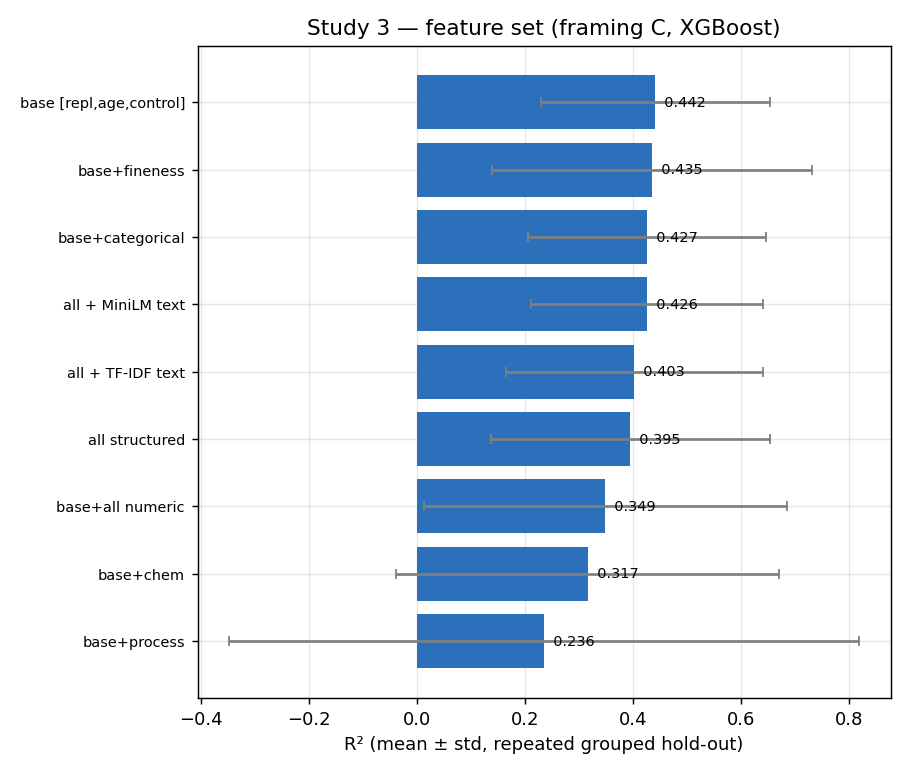
\includegraphics[width=0.6\linewidth]{abl_features.png}
  \caption{Feature-set ablation: parsimony wins (repeated grouped hold-out, mean\,$\pm$\,std).}
  \label{fig:ablfeat}
\end{figure}

% ============================================================================
\section{Final Model and Results}
\label{sec:final}

\paragraph{Features used (framing C).} The final model takes exactly three inputs---no
RHA chemistry, physical, or processing features are included, and Study~3 above is the
evidence for why (every added feature group made generalization \emph{worse} at
$n=23$ papers):

\begin{center}\small
\begin{tabular}{lll}
\toprule
Feature & Meaning & Monotone constraint \\
\midrule
\texttt{replacement\_pct} & RHA cement-replacement level of the blend row (0--100\%) & none \\
\texttt{age\_days} & Curing age at which strength is measured (days) & non-decreasing \\
\texttt{ctrl\_strength} & The \emph{same paper's own} 0\% (control) compressive & non-decreasing \\
 & strength at the matching curing age (MPa) & \\
\bottomrule
\end{tabular}
\end{center}

\noindent The target is \texttt{strength\_mpa}, the RHA-blend row's own compressive
strength. \texttt{ctrl\_strength} is looked up per \texttt{(paper\_id, age\_days)} from
that paper's own 0\%-replacement rows (Section~\ref{sec:final} onward always assumes it
is known at inference time, since it is the paper's own OPC baseline, not a property of
the RHA blend being predicted). Combining these three features with monotone
constraints and a light grouped hyper-parameter search yields a deliberately shallow
model (\texttt{max\_depth}=2, \texttt{learning\_rate}=0.03, 300 trees). Its performance
is

\begin{center}\small
\begin{tabular}{lccc}
\toprule
 & \R{} & RMSE (MPa) & MAE (MPa) \\
\midrule
\textbf{Final model} (repeated grouped hold-out) & $\mathbf{0.50\pm0.20}$ & $\mathbf{14.9}$ & $\mathbf{10.1}$ \\
Mean baseline & $-0.31$ & $24.0$ & $17.4$ \\
\bottomrule
\end{tabular}
\end{center}

Figure~\ref{fig:pva} shows out-of-fold predictions. Note that its panel title reports
\R{}~$=0.63$, MAE~$=9.4$\,MPa, which is \emph{not} the headline number above: the
scatter comes from a single 5-fold \texttt{GroupKFold} pass whose out-of-fold
predictions are pooled into one \R{} over all 335 rows, whereas the table reports the
mean of 40 grouped hold-outs that each train on fewer papers (70\% vs 80\%) and are
scored split-by-split. The pooled single-pass figure is the more optimistic of the two;
we quote the repeated hold-out as the honest estimate and show the pooled predictions
only because they give one prediction per row to plot.

The model tracks normal-strength concrete well but systematically
\emph{under-predicts} the high end. Note that the 1--205\,MPa span quoted in Study~1
describes framing~A; framing~C is evaluated on the 335 blend rows of 23 papers that
also report a 0\% control, and that subset reaches 186\,MPa. Within it there is
\textbf{exactly one} paper above 120\,MPa (8 points, 120--186\,MPa), and the model's
predictions saturate near 90\,MPa there, under-shooting by 70\,MPa on average. The
corpus does contain a second, even stronger paper---it holds the 205\,MPa maximum---but
it reports no control rows at all and is therefore excluded from framing~C entirely,
which is part of why 44 papers reduce to 23 here. With a single high-strength group in
the evaluated set, grouped validation always places it wholly in the test fold, so the
model has never seen a UHPC example when it is scored---an honest and interpretable
failure mode, but one driven by a single group rather than by a subpopulation. That
tail is also what pulls
the residual distribution (Figure~\ref{fig:resid}) slightly negative: residuals are
centred near zero (mean $-2.7$\,MPa, median $-2.2$\,MPa) but carry a long left tail
reaching $-100$\,MPa, all of it from that one paper. Feature importance
(Figure~\ref{fig:imp}) confirms that control strength (0.74) and curing age (0.17)
carry most of the signal, with replacement level (0.09) modulating on top.

\begin{figure}[H]
  \centering
  \begin{subfigure}{0.4\textwidth}
    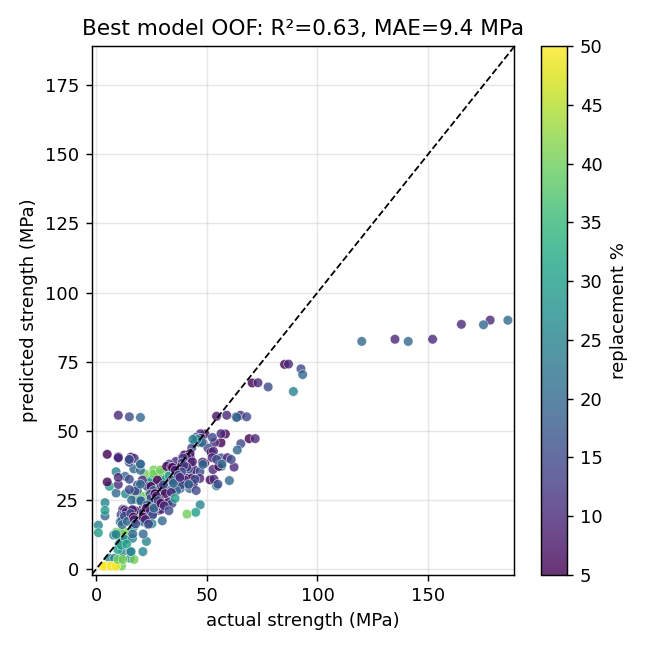
\includegraphics[width=\linewidth]{pred_vs_actual.png}
    \caption{Out-of-fold predictions.}
    \label{fig:pva}
  \end{subfigure}\hfill
  \begin{subfigure}{0.57\textwidth}
    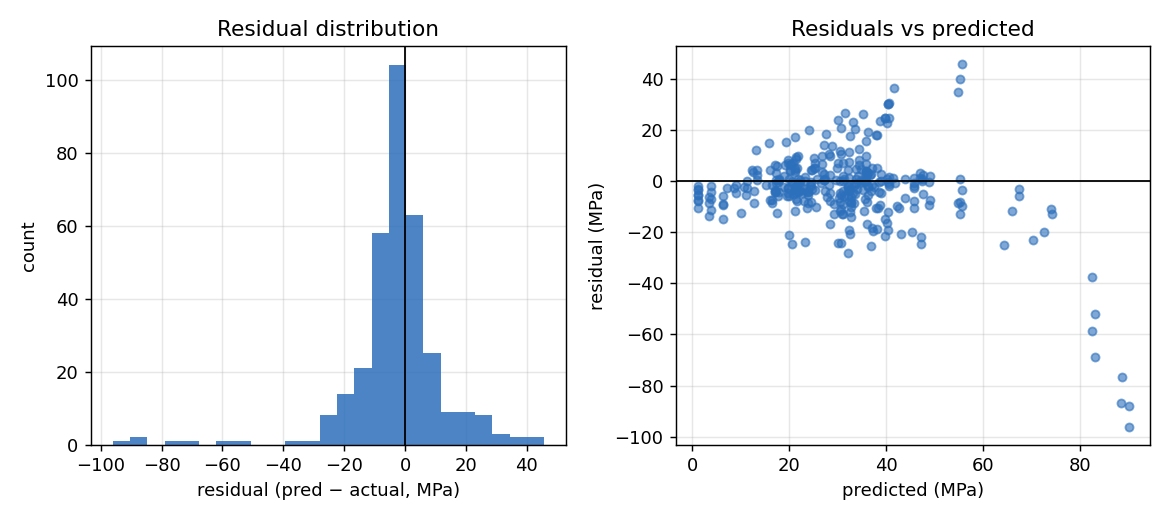
\includegraphics[width=\linewidth]{residuals.png}
    \caption{Residual diagnostics.}
    \label{fig:resid}
  \end{subfigure}
  \caption{Final model behaviour, from a single pooled 5-fold \texttt{GroupKFold} pass
  (\R{}~$=0.63$ pooled, versus the $0.50\pm0.20$ repeated-hold-out estimate quoted in
  the table above). Colour encodes replacement level. The dashed line is the ideal
  $y=x$; the points falling far below it at the right of (a) are the single UHPC paper.}
\end{figure}

\begin{figure}[H]
  \centering
  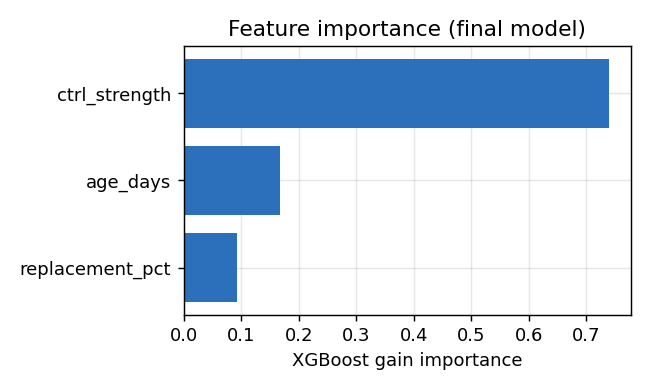
\includegraphics[width=0.55\textwidth]{feature_importance.png}
  \caption{Feature importance of the final model. The paper's control strength and the
  curing age dominate; replacement level provides the RHA-specific modulation.}
  \label{fig:imp}
\end{figure}

% ============================================================================
\section{Predicting the Optimal Replacement Level}
\label{sec:opt}
We derive the optimum as the replacement level that maximizes the predicted 28-day
strength curve of the final model, evaluated on held-out papers, and also test a direct
per-paper regressor. Neither beats simply predicting the corpus-mean optimum: on the 20
held-out papers with a reported optimum the argmax approach gives
MAE~$=4.75$ percentage points against a mean-baseline of $3.45$, and the direct
regressor gives $6.5$ against its own baseline of $5.3$ over 43~papers.

Figure~\ref{fig:opt} shows why, and the failure is starker than ``fails to beat the
baseline'' suggests: \textbf{the argmax model returns the same value, 7.5\%, for every
one of the 21 held-out papers}. It is a constant predictor, and a miscalibrated one,
since the corpus mean is 11.5\%. This is a direct consequence of the final model's
structure---it is monotone and non-decreasing in control strength and age, and with
\texttt{max\_depth}=2 there is almost no interaction between replacement level and the
other two inputs, so changing a paper's control strength shifts the predicted strength
curve vertically without moving the location of its maximum. Every paper therefore
inherits the same argmax.

The reported optima it is scored against are themselves concentrated but not tight:
75\% of papers fall in 10--15\% (mean 11.5\%, median 10\%), yet the full range runs
0--20\% with a standard deviation of 4.6 points. A constant-11.5\% prior already
achieves MAE 3.45, so beating it requires resolving paper-to-paper shifts of a few
percentage points---and with 20--43 labelled papers, and an interior optimum present in
only 42\% of them (Section~3), that signal is not available. Predicting the optimum is
best treated as an open problem on this corpus rather than a solved output.

\begin{figure}[H]
  \centering
  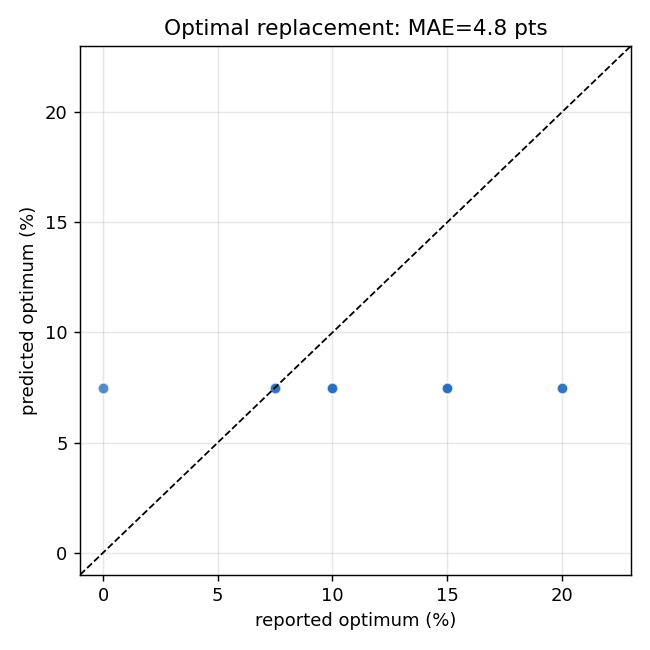
\includegraphics[width=0.5\textwidth]{optimum_scatter.png}
  \caption{Predicted vs reported optimal replacement level. The predictions form a
  horizontal line: the model emits a constant 7.5\% for every held-out paper, below the
  11.5\% corpus mean, and so loses to the mean prior it is compared against.}
  \label{fig:opt}
\end{figure}

% ============================================================================
\part*{Part II --- Sensitivity to the UHPC-Regime Outliers}
\label{sec:part2}

Sections~\ref{sec:final}--\ref{sec:opt} flagged, but did not remove, the two papers
responsible for the corpus's 1--205\,MPa span. This part removes them and re-measures
both target framings, to separate ``the model degrades on UHPC'' from ``the model is
fine once UHPC is taken out of scope.''

\section{Which Papers, and Why}
\label{sec:part2-cutoff}
The cutoff is applied at the \emph{paper} level, not the row level: a paper is dropped
in full---every replacement level, every curing age---if its \textbf{maximum} reported
compressive strength exceeds \textbf{120\,MPa}. This threshold is not a round-number
guess; it sits in a genuine gap in the data. Of the 44 papers, only two ever cross it,
and the next-highest paper after them tops out at exactly 100.0\,MPa (Table~\ref{tab:cutoff}).

\begin{center}\small
\begin{tabularx}{\linewidth}{@{}clcX@{}}
\toprule
ID & Title (abridged) & Max str. & Why it is out of scope \\
\midrule
17 & ``...to produce ultra high performance concrete'' & 205.5\,MPa &
  Explicitly UHPC. $w/b=0.15$--$0.23$ vs.\ $\approx0.35$--$0.50$ for the rest of the
  corpus. Strength rises smoothly $51\to205.5$\,MPa with age---internally
  consistent, just a different mix-design regime (silica fume / superplasticizer /
  very low $w/b$), not ordinary RHA concrete. \\[0.4em]
36 & ``Analysis of the effects of RHA on hydration...'' & 186.0\,MPa &
  Reports 125--135\,MPa at \textbf{1 day} of curing, including for its own 0\%
  control---not physically plausible at any $w/b$. Every value is flagged
  \texttt{is\_range=True} (read off a graph axis, not a table), consistent with a
  mis-read scale rather than genuine UHPC. \\
\bottomrule
\end{tabularx}
\captionof{table}{The two papers removed by the 120\,MPa cutoff, and the highest
strength reported by any of the 42 papers kept: 100.0\,MPa.}
\label{tab:cutoff}
\end{center}

This directly tests the diagnosis already made in Section~\ref{sec:final}: that
framing~A's negative \R{} comes from mixing mortars, normal concrete and UHPC on one
strength scale, and that framing~C is largely insulated from this because it
conditions on each paper's own control strength. Paper~17 was never in framing~C to
begin with (it reports no 0\% control); paper~36 was one of its 23 papers.

\paragraph{Reproducibility check.} Both sides below were re-run with the identical
model class and hyper-parameter grid as Sections~\ref{sec:final}--\ref{sec:opt}. The
unfiltered ``before'' run here reproduces the Section~\ref{sec:final} headline almost
exactly (\R{}~$=0.503\pm0.197$, RMSE$=14.90$, MAE$=10.02$ vs.\ the original
\R{}~$=0.50\pm0.20$, RMSE$=14.9$, MAE$=10.1$), confirming the numbers below are
directly comparable to the rest of this report.

\section{Results With and Without the UHPC Papers}
\label{sec:part2-results}

\begin{center}\small
\begin{tabular}{lccc}
\toprule
\textbf{Framing A} (absolute strength, no baseline info) & \R{} & RMSE (MPa) & MAE (MPa) \\
\midrule
With UHPC papers (44 papers, 756 rows, 1--205.5\,MPa) & $-0.43\pm0.78$ & $29.5$ & $20.2$ \\
Without UHPC papers (42 papers, 706 rows, 1--100\,MPa) & $\mathbf{+0.08\pm0.23}$ & $\mathbf{17.1}$ & $\mathbf{13.0}$ \\
\bottomrule
\end{tabular}
\end{center}

\begin{center}\footnotesize
\begin{tabular}{lcccc}
\toprule
\textbf{Framing C} (tuned, blend $\mid$ control) & \R{} & RMSE (MPa) & MAE (MPa) & OOF \R{} \\
\midrule
With UHPC papers (23 papers, 335 rows) & $0.50\pm0.20$ & $14.9$ & $10.0$ & $0.63$ \\
Without UHPC papers (22 papers, 327 rows) & $\mathbf{0.52\pm0.16}$ & $\mathbf{11.4}$ & $\mathbf{8.6}$ & $0.60$ \\
\bottomrule
\end{tabular}
\end{center}

\begin{center}\small
\begin{tabular}{lcc}
\toprule
\textbf{Optimal replacement} (argmax, 28-day, held-out papers) & MAE (pts) & Mean-baseline (pts) \\
\midrule
With UHPC papers (20 papers) & $4.75$ & $3.45$ \\
Without UHPC papers (20 papers) & $4.75$ & $3.45$ \\
\bottomrule
\end{tabular}
\end{center}

\section{Discussion}
\label{sec:part2-discussion}
The two framings respond differently, and the difference is diagnostic rather than
incidental. \textbf{Framing A flips sign}: \R{} crosses from $-0.43$ to $+0.08$, and
RMSE/MAE fall by 42\% and 36\% respectively (29.5$\to$17.1\,MPa; 20.2$\to$13.0\,MPa). A
model that is never told a paper is UHPC has no way to know it should predict
180\,MPa instead of 40\,MPa for a nominally similar input row; once the two UHPC-regime
papers are removed, the remaining 42 papers occupy one coherent strength scale
(1--100\,MPa) and the same features that were noise before now carry signal. \R{}~$=0.08$
is still weak in absolute terms---framing~A was never going to become the recommended
model---but the sign flip alone confirms the diagnosis.

\textbf{Framing C improves modestly but genuinely}: \R{} rises from $0.50$ to $0.52$
with a visibly tighter spread across repeats ($\pm0.20\to\pm0.16$), and RMSE/MAE both
drop by double digits (14.9$\to$11.4\,MPa, $-24\%$; 10.0$\to$8.6\,MPa, $-14\%$). This is
smaller than framing~A's swing, exactly as Section~\ref{sec:final} predicted:
conditioning on the paper's own control strength already absorbs most of the
cross-paper scale variation that framing~A is exposed to raw, so removing the outlier
papers here mostly trims a noisy, hard-to-fit paper (36) from a 23-paper set rather than
unlocking new signal. One number moves the other way---the pooled single-pass OOF
\R{} used for the prediction-scatter figure drops slightly ($0.63\to0.60$)---which is
expected: that figure is a single 5-fold split, more sensitive to exactly which papers
land in which fold when there are only 22--23 of them, and is not the metric either
number in the table above is drawn from. The optimal-replacement argmax MAE is
\emph{exactly} unchanged (4.75 points against an unchanged 3.45-point baseline, both
sides): neither dropped paper had a usable reported optimum, so that evaluation set of
20 papers is identical before and after.

The practical conclusion is that \textbf{outlier removal and the control-strength
reframing are two different fixes for the same underlying problem}, and only one of
them is needed if framing~C is what will be deployed. Framing~A's improvement after
cleaning is useful mainly as confirmation that the corpus is well-behaved once UHPC is
excluded, not as a replacement for framing~C, which remains the stronger predictor
either way ($0.50$--$0.52$ \R{} vs.\ $0.08$ at best). If the eventual goal includes UHPC-range
predictions, the two removed papers should be re-added as a separate, explicitly
labelled regime (e.g.\ a categorical ``mix class'' feature) rather than silently
dropped, since 8--38 data points is too little to train a UHPC-specific model on its
own; for the conventional-concrete regime this report otherwise targets, dropping them
is the right call.

% ============================================================================
\section{An LLM Ablation: Does Control Strength Matter Across Model Families?}
\label{sec:part2-opus}

Sections~\ref{sec:final} and Study~1 (Table~\ref{tab:s1}) established, with a trained
regressor, that supplying a paper's own 0\% control strength is what makes RHA-blend
strength learnable at all. Two independent LLM experiments ask the same question with
no gradient-boosted model in the loop at all: given the same tabular rows, can a
general-purpose LLM infer compressive strength from the paper's inputs alone, and does
it too depend on being handed the control strength?

\paragraph{Setup.} Six papers were held out at the \emph{paper} level---P036, P022,
P007, P030, P054 and P064, none seen in training---giving a fixed benchmark of
\textbf{57 test points} shared identically by both conditions and both models, so the
ablation isolates one variable:
\begin{description}\itemsep2pt
  \item[WITH\_CONTROL] the model is given the paper's 28-day 0\% control strength as an
        input feature, exactly as framing~C does for the ML model.
  \item[NO\_CONTROL] control strength is withheld; only the RHA/mix inputs remain.
\end{description}

\paragraph{Two models.} \textbf{Claude Fable} was evaluated externally (results as
reported); \textbf{gpt-oss:120b-cloud} (OpenAI's open-weight $\sim$117B-parameter
model, MXFP4-quantized, accessed through Ollama's cloud proxy) was run for this report
directly against the identical ground truth, one Ollama call per test paper per
condition (12 calls total), each given that paper's held-out rows plus the \emph{entire}
condition's training CSV as in-context reference data, prompted to return a strict JSON
array of predictions. gpt-oss was reached only after two earlier choices failed:
DeepSeek-R1 8B run locally took 10+ minutes for a single call at this context length on
an 8\,GB laptop GPU (impractical for 12 calls), and \texttt{kimi-k2.6:cloud} returned
402 Payment Required (a paid ollama.com plan). gpt-oss:120b-cloud is free-tier
accessible, cloud-hosted, and answered every call in 20--100\,s. One call (NO\_CONTROL,
paper P007) initially degenerated---the model echoed the four \emph{age} values back
verbatim instead of predicting strength; it was retried once and produced a normal,
non-degenerate answer, which is what is reported below. Because the two models were
evaluated under different prompting protocols (Fable's exact prompt is not available to
us), this is not a controlled head-to-head between Fable and gpt-oss---it is two
\emph{separate} within-model ablations that happen to share the same benchmark, and
both are compared only against themselves (WITH\_ vs NO\_CONTROL), not against each
other.

\subsection{Overall Result}
\begin{center}\small
\begin{tabular}{lrrrr}
\toprule
Condition & \R{} & RMSE (MPa) & MAE (MPa) & Bias (MPa) \\
\midrule
\rowcolor{green!12}Fable, WITH\_CONTROL & $\mathbf{0.877}$ & $\mathbf{8.79}$ & $\mathbf{5.84}$ & $-2.21$ \\
Fable, NO\_CONTROL & $0.392$ & $19.50$ & $12.83$ & $-6.25$ \\
\rowcolor{green!12}gpt-oss:120b, WITH\_CONTROL & $\mathbf{0.887}$ & $\mathbf{8.41}$ & $7.17$ & $-1.48$ \\
gpt-oss:120b, NO\_CONTROL & $0.487$ & $17.92$ & $12.78$ & $-6.82$ \\
\midrule
Final ML model (Section~\ref{sec:final}, for reference) & $0.50\pm0.20$ & $14.9$ & $10.1$ & --- \\
\bottomrule
\end{tabular}
\end{center}

\noindent Both LLMs move the same way. For Fable, control strength lifts \R{} by
$+0.485$ and cuts RMSE/MAE by roughly \textbf{55\%}. For gpt-oss, control strength
lifts \R{} by $+0.400$ and cuts RMSE by \textbf{53\%} (17.92$\to$8.41\,MPa) and MAE by
\textbf{44\%} (12.78$\to$7.17\,MPa)---the same qualitative effect Study~1 found for the
ML model, now reproduced independently by \emph{two} completely different LLMs. The ML
row is included only as context, \emph{not} as a matched comparison: it is a repeated
grouped hold-out averaged over 40 different 70/30 paper splits, whereas all four LLM
rows are single evaluations on one fixed six-paper split. Neither LLM's WITH\_CONTROL
number should be read as ``beats the ML model''---the honest claim in both cases is the
ablation \emph{within} that model, which needs no such caveat because both conditions
share the identical test papers.

\subsection{Result by Compressive-Strength Category}
\label{sec:part2-opus-bins}
The dataset's own three strength regimes (Low $<30$\,MPa, Middle $30$--$60$\,MPa, High
$\geq60$\,MPa) split the 57 test points 24/18/15 and reveal where control strength
actually earns its keep, for both models.

\begin{center}\footnotesize
\begin{tabular}{lrrrrrrrr}
\toprule
& \multicolumn{4}{c}{NO\_CONTROL (MAE / Bias, MPa)} & \multicolumn{4}{c}{WITH\_CONTROL (MAE / Bias, MPa)} \\
& \multicolumn{2}{c}{Fable} & \multicolumn{2}{c}{gpt-oss} & \multicolumn{2}{c}{Fable} & \multicolumn{2}{c}{gpt-oss} \\
Regime ($N$) & MAE & Bias & MAE & Bias & MAE & Bias & MAE & Bias \\
\midrule
Low, $<30$ (24) & $7.31$ & $+7.31$ & $7.02$ & $+5.86$ & $3.84$ & $+3.70$ & $5.59$ & $+5.26$ \\
Mid, $30$--$60$ (18) & $3.19$ & $-1.87$ & $5.21$ & $-3.51$ & $3.85$ & $-2.89$ & $7.51$ & $-4.14$ \\
High, $\geq60$ (15) & $33.22$ & $-33.22$ & $31.09$ & $-31.09$ & $\mathbf{11.43}$ & $-10.85$ & $\mathbf{9.30}$ & $-9.09$ \\
\bottomrule
\end{tabular}
\end{center}

\noindent The pattern is sharp, matches the UHPC discussion of
Section~\ref{sec:part2-cutoff}, and now holds for \emph{both} LLMs independently:
\textbf{without} control strength, both models are reasonably behaved in the low and
middle regimes but collapse on the high regime, under-predicting by a mean of
$31$--$33$\,MPa---neither model has any way to know a given paper's own strength
ceiling, so both regress toward the corpus-typical range. \textbf{With} control
strength, high-regime MAE falls to $9.30$--$11.43$\,MPa (a $\sim$65--70\% reduction)
because the model is now told, explicitly, which papers are high-baseline. The low and
middle regimes---already easy without any baseline signal---show smaller, noisier
shifts (gpt-oss's mid-regime MAE actually rises slightly, $5.21\to7.51$, well within the
noise of a 15--18-point evaluation). This mirrors exactly why framing~C outperforms
framing~A for the XGBoost model: the hard part of this corpus was never the RHA effect
itself, it is locating each paper's baseline strength level, and \emph{any} sufficiently
capable predictor---tree-based, or either of two unrelated LLM families---needs that
baseline supplied to do well outside the middle of the strength range.

\subsection{Where It Still Fails: Paper P064}
Both models and both conditions agree on the single hardest case. Paper P064 (6 points,
high replacement/high strength) is the worst-or-tied-worst per-paper error everywhere:

\begin{center}\small
\begin{tabular}{lrrrr}
\toprule
& \multicolumn{2}{c}{MAE, NO\_CONTROL} & \multicolumn{2}{c}{MAE, WITH\_CONTROL} \\
Paper & Fable & gpt-oss & Fable & gpt-oss \\
\midrule
P064 (hardest) & $47.95$ & $33.70$ & $21.37$ & $12.89$ \\
next-worst & $23.40$ (P054) & $29.34$ (P054) & $4.81$ (P054) & $7.68$ (P007) \\
\bottomrule
\end{tabular}
\end{center}

\noindent Control strength shrinks P064's error substantially for both models (Fable
$47.95\to21.37$; gpt-oss $33.70\to12.89$), but it remains the largest per-paper error by
a wide margin in every configuration. At 28 days, NO\_CONTROL predictions undershoot
this paper's true 90--111\,MPa range by 60--70\,MPa (Fable) or land in the 40s-to-60s
(gpt-oss)---even with age and replacement given, neither model can guess this paper's
unusually high strength scale without being told it. This is the same failure mode
already documented for the final ML model in Section~\ref{sec:final} (systematic
under-prediction at the high end, worst on the corpus's most extreme paper)---further
evidence that the limitation is in the \emph{data} (a handful of unusually strong papers
with no comparable neighbors to generalize from), not specific to any one modeling
approach.

\subsection{Summary}
Two unrelated LLMs, evaluated independently and under different prompting protocols,
replicate this report's central empirical claim, first established with a
three-feature, monotone, depth-2 XGBoost tree: \textbf{a paper's own control strength
is the dominant signal for predicting RHA-blend compressive strength, and its absence
is felt almost entirely at the high-strength end of the corpus.} That three completely
different predictors---a gradient-boosted tree and two general-purpose LLMs from
different vendors---land on the same qualitative conclusion, on the same held-out
papers, is considerably stronger evidence for that claim than any single result alone.

\end{document}
